\documentclass{jknotes}
\usepackage{../joshkirklin}

\tikzset{
    partial ellipse/.style args={#1:#2:#3}{
        insert path={+ (#1:#3) arc (#1:#2:#3)}
    }
}

\setmathfont{Latin Modern Math}
\setmathfont{GFS NeoHellenic Math}[range=bfsfup/{greek,Greek}->it]
\setmathfont{GFS NeoHellenic Math}[range=sfup/{latin,Latin}->it]

\usetikzlibrary{intersections, pgfplots.fillbetween}
\begin{document}

\institution{Cambridge Part III Maths}
\title{Fluid Dynamics of the Solid Earth}
\lecturer{Dr. Jerome Neufeld}
\notetaker{Charles Powell}
\date{Lent 2020}

\maketitle
\suggestionsspiel
\tableofcontents

\lecture{21/01/21}
\section{Introduction}
The course will use the wealth of observations of the solid Earth to motivate
mathematical models of the physical processes governing its evolution. The
dynamic evolution is governed by a rich variety of physical processes occuring
on a wide range of length and time scales. 

\begin{itemize}
	\item The Earth's core is formed by the solidifcation of a mixture of
		molten iron and various light elements, a process which drives
		predominantly compositional convection in the liquid outer core, thus
		producing the geodynamo responsible for the Earth's magnetic field. 
	\item On million year timescales, the solid mantle convects, and as it
		upwells to the surface it partially melts leading to the volcanism. 
	\item At the surface, convection drives the motion of brittle plates which
		are responsible for the Earth's topography as can be felt and imaged
		through the seismic record (figure~\ref{fig:seismology})
	\item In the Earth's surface, fluids flow through poroous rocks, for
		example groundwater aquifers which feed streams and rivers which erode
		the solid surface.
	\item On the Earth's surface, similarity physical processes of viscous and
		elastic deformation coupled to phase changes govern the evolution of
		the Earth's cryosphere, from the solidification of sea ice to the flow
		of glacial ice over land and ice shelves over the ocean.
\end{itemize}
\begin{figure}
	\centering
	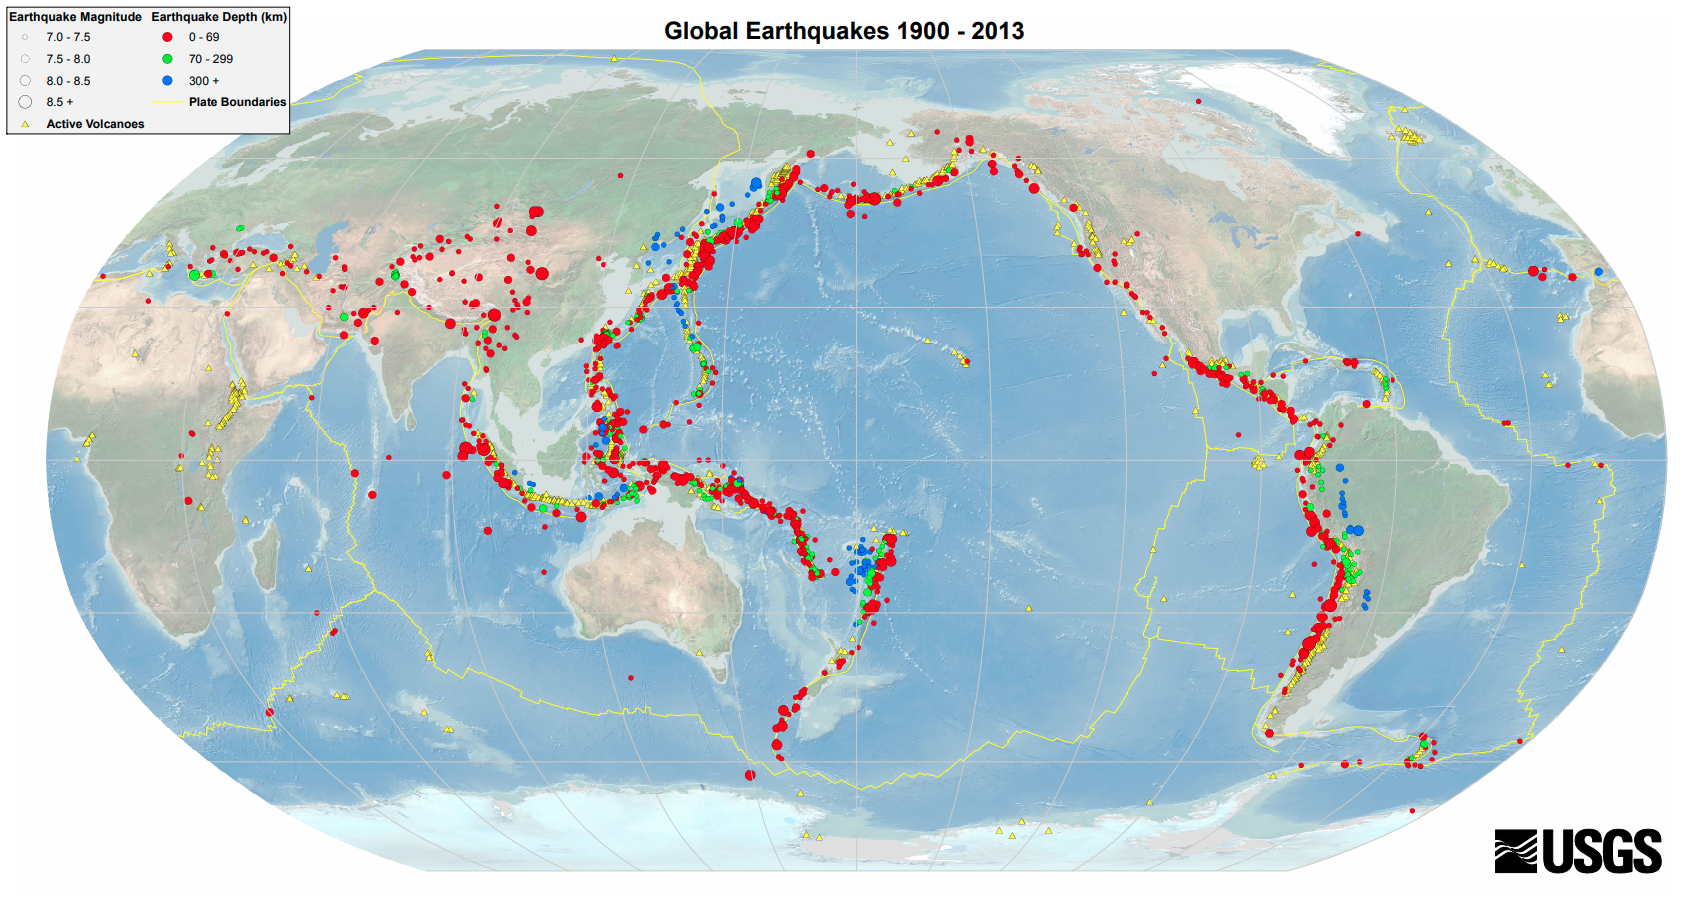
\includegraphics[width=\textwidth]{earthquakes.png}
	\caption{Map of global earthquakes, visibly localised to tectonic plate
	boundaries.}
	\label{fig:seismology}
\end{figure}

Predominantly, the mathematics is of slow viscous flows. Topics include the
onset and scaling of convection, the coupling of fluid motions with changes of
phase at a boundary, the thermodynamic and mechanical evolution of
multicomponent or multiphase systems, the coupling of fluid flow and elastic
flexure or deformation, and the flow of fluids through porous materials. 

\section{Half-space cooling of the oceanic plates (mid-ocean ridges)}
The bottom surface of Earth's oceans, particularly clear in the Atlantic
ocean, has a large scale structure in which the middle of the ocean (the
\emph{mid-ocean ridge}) is shallower than regions closer to the continents.
The mid-ocean ridge forms as a result of separating tectonic plates. We know
that the plates move apart here due to magnetic anomalies forming `stripes' of
alternating polarity. The quasi-periodic flipping of the Earth's magnetic
polarity allows dating of the stripes. The plates are driven apart by
convection of the Earth's mantle.

We wish to form a model describing the depth of the ocean floor near mid-ocean
ridges. First we estimate the temperature field. Consider an idealised model
with a flat surface (for now), observed plate spreading rate $U$, surface
temperature $T_0$, deep mantle temperature $T_1$.
The temperature field is described by the advection-diffusion equation
\begin{equation}
	\rho c_p \left(\frac{\partial T}{\partial t} + \symbf{u}\cdot\nabla T
	\right) = \nabla \cdot (k \nabla T)
\end{equation}
where $c_p$ is specific heat capacity, $k$ is thermal conductivity, $\rho$ is
density, all assumed constant. For simplicity, we combine these constants into
the thermal diffusivity $\kappa = k/\rho c_p$. Then
\begin{equation}
	\frac{\partial T}{\partial t} + \symbf{u}\cdot\nabla T
	 = \kappa \nabla^2 T
\end{equation}

\begin{figure}
	\begin{center}
	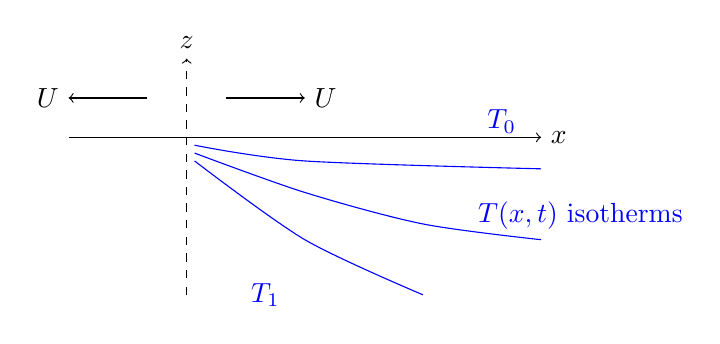
\begin{tikzpicture}
		\draw[->] (-3, 0) -- (3, 0) node[right] {$x$};
		\draw[dashed,->] (-1.5, -2) -- (-1.5, 1) node[above] {$z$};
		\draw[->] (-1, 0.5) -- (0, 0.5) node[right] {$U$};
		\draw[->] (-2, 0.5) -- (-3, 0.5) node[left] {$U$};
		\draw[smooth,blue] plot coordinates {(-1.4, -0.1) (0, -0.3) (3,
		-0.4)};
		\draw[smooth,blue] plot coordinates {(-1.4, -0.2) (0, -0.7) (1.5,
			-1.1) (3, -1.3)};
		\draw[smooth,blue] plot coordinates {(-1.4, -0.3) (0, -1.3) (1.5,
		-2)};
		\draw[blue] (3.5, -1) node {$T(x,t)$ isotherms};
		\draw[blue] (2.5, 0.2) node {$T_0$};
		\draw[blue] (-0.5, -2) node {$T_1$};
	\end{tikzpicture}
	\caption{Schematic diagram of mid-ocean ridge spreading and mantle
	temperature isotherms.}
\end{center}
\end{figure}


We wish to find the steady state profile with $\partial_t = 0, \symbf{u} = U
\hat{\symbf{x}}$ where $U$ is constant. Note that far from the ridge axis, the
thickness of the plate is much smaller than the extent of the plate. Hence in
terms of scalings, $z \ll x$ and we may neglect the $\partial_x^2$ component
of $\nabla^2$. We have
\begin{equation}
	U \frac{\partial T}{\partial x} = \kappa \left( \frac{\partial^2
	T}{\partial x^2} + \frac{\partial^2 T}{\partial z^2}\right) \approx \kappa
	\frac{\partial^2 T}{\partial z^2}
	\label{eq:temp}
\end{equation}
The scaling given by this equation is $U\Delta T / x \sim \kappa \Delta T /
z^2$ where $\Delta T = T_1 - T_0$ is the natural temperature scale. There is
no natural lengthscale, so we use that given by the advection-diffusion
equation:
\begin{equation}
	z \sim \sqrt{\frac{\kappa x}{U}}
\end{equation}

We can proceed by finding a self-similar solution with similarity variable
\begin{equation}
	\eta = \frac{z}{2\sqrt{\frac{\kappa x}{U}}}
\end{equation}
and seek solutions of the form
\begin{equation}
	\theta = \frac{T - T_0}{T_1-T_0} = \theta(\eta)
\end{equation}
Using the variables $\eta, \theta$, \eqref{eq:temp} becomes
\begin{align}
	-U\Delta T \frac{\eta}{2x} \theta_\eta &= \frac{\kappa \Delta T}{4
	\frac{\kappa x}{U}} \theta_{\eta\eta}\\
		\implies \theta_{\eta\eta} + 2\eta\theta_\eta &= 0
\end{align}
We can integrate directly to get $\theta_\eta = ae^{-\eta^2}$, which gives
\begin{equation}
	\theta = b + a \int_0^\eta e^{-y^2} \, \diffd y
\end{equation}
The boundary conditions are $\theta(0) = 1$ and $\theta(\infty) = 1$ based on
the definitions of $T_0$ and $T_1$. The thermal structure away from the ridge
is then
\begin{equation}
	T = T_0 + (T_1-T_0) \erf\left( \frac{z}{2\sqrt{\frac{\kappa x}{U}}}\right)
\end{equation}
where the error function $\erf$ and its complement erfc are defined by
\begin{align}
	\erf(x) &= \frac{2}{\sqrt{\pi}} \int_0^x e^{-y^2} \, \diffd y \\
	\text{erfc}(x) &= 1 - \erf(x)
\end{align}


\end{document}
